\documentclass[circuitt, largebox]{efrei_report_card}

\author{Jacques Soghomonyan}
\title{Rapport Projet}
\subtitle{Microcontrôleur en VHDL}

\graphicspath{ {./images} }

\usepackage{capt-of}

\begin{document}
  \maketitle

  \tableofcontents
  \pagebreak

  \note{Les images de simulation sont parfois assez petite et un zoom peut être nécessaire pour les comprendre.}

  \exercise{Introduction}{
    \question[]{}{
      Ce projet a pour but de nous introduire au monde des cartes programmables FPGA.

      Pour ce faire nous avons programmé, en VHDL, une architecture simple de microcontrôleur.
      Ici, nous allons détailler les aspects techniques de toutes les composantes.

      \medskip

      L'implémentation des composants est traité dans ce rapport mais, le code étant assez explicite, nous ne nous attarderons pas plus que ça sur le code.

      \medskip

      J'ai décidé de donner des noms très verboses aux signaux pour mieux comprendre et identifier les problèmes.
      C'est pourquoi ils diffèrent de ceux donné dans le sujet.
    }
  }

  \exercise{Plan d'attaque.}{
    \question{Avant-gout.}{
      Nous devons diviser le problème pour qu'il convienne au modèle entité de VHDL.

      L'énoncé est exhaustif quant à la manière de faire et les éléments à prendre en compte pour construire le système.
      \medskip

      Dans le sujet, un schéma nous est donné. J'ai décidé d'en diverger un peu\footnote{
        Le schéma simplifié, montrant les nouvelles connexions, peut être trouvé dans le fichier \textbf{project-schema.pdf}.

        Le schéma n'est pas légendé, mais les entrées, sorties, dimensions des ports, nom des ports sont identifiables.
        Même s'il n'est pas à jour, il permet de visualiser l'agencement du projet.
  
        Il est fait pour être lu en tandem avec le sujet original.
      }.
      En effet, certaines connexions semblaient redondantes p.~ex.~connexion de l'horloge à l'interconnexion.
      De plus, d'autres étaient implicites p.~ex.~les \textit{enable} des \textit{buffer}.
    }

    \question{Outils auxiliaires.}{
      Pour ce projet, j'ai décidé d'utiliser des outils auxiliaires pour faciliter le flux de travail.

      \begin{description}
        \item[GNU Make] Un outil d'automatisation de construction de projet. 
        Toutes les commandes d'élaboration et des tests unitaires sont déléguées à ce système.
        \item[cocotb] Un outil aidant l'écriture de tests unitaires\footnote{J'ai originalement rédigé des tests en vhdl, mais j'ai ultimement décidé de les refaire en python. Les originales sont encore là.} avec des scripts python.
      \end{description}
    }

    \question{Les composants.}{
      Voici la liste des composants, traduis par des entités en VHDL, de notre système.

      \begin{itemize}
        \item Le buffer
        \item L'unité arithmétique logique
        \item Le bloque d'instruction
        \item L'interconnexion
      \end{itemize}

      Nous élaborerons sur l'implémentation technique dans la partie qui suit.
    }
  }

  \pagebreak
  \exercise{L'implémentation.}{
    \question{Arborescence du projet.}{
      Les composants sont nommés en anglais, parfois mal, comme avec le \textbf{dbus}, représentant l'interconnexion.
      Mais par soucis de complexité de tout changer, j'ai laissé les noms donnés au début du projet.

      Tous les composants nommés au-dessus sont stockés dans des dossiers éponymes\footnote{en anglais}.

      \medskip
      
      Dans les dossiers, on peut retrouver, en général :
      
      \begin{itemize}
        \item Un fichier VHDL principal contenant l'entité en question et son architecture.
        \item Un fichier VHDL générant le signal visualisable.
        \item Un fichier VHDL contenant les tests unitaires pour l'entité.
        \item Un fichier python contenant également des tests unitaires pour l'entité.
        \item Un dossier contenant les signaux visualisables, nommé \textbf{waves/}.
        \item Et enfin un \textit{makefile}, utilisé pour lancer les tests et générer les signaux pour l'entité.
      \end{itemize}

      \medskip

      Dans la racine du répertoire, un \textit{makefile} lance tous les tests de tous les composants du système et synthétise
      le composant nommé \textbf{microcontroler}, la synthèse de toutes les entités. 
    }

    \question{nbuffer}{
      Le buffer est l'élément le plus utilisé du projet.

      En effet, c'est l'entité derrière :
      \begin{itemize}
        \item out\_sel\_buf
        \item fn\_sel\_buf
        \item carries\_buf
        \item a\_buf
        \item b\_buf
        \item cache1\_buf
        \item cache2\_buf
      \end{itemize}

      C'est un buffer assez simple.
      Le composant renvoie l'entrée sur front montant d'horloge.
      
      Il possède aussi deux signaux de contrôle.
      
      Le signal \textbf{enable}, qui permet une mémoire, la sortie ne change que si le signal est actif.
      
      Le signal \textbf{reset}, qui remet la sortie à zéro asynchroniquement.

      \note{
        Les signaux originalement nommés \textbf{SR\_IN\_L} et \textbf{SR\_IN\_R}, sont devenus un seul buffer nommé \textbf{carries\_buf}.
        
        De plus, les signaux nommés \textbf{SR\_OUT\_L} et \textbf{SR\_OUT\_R}, sont juste un vecteur de taille 2 en sortie du microcontrôleur.
      }
    }
    \question{alu}{
      L'alu agit asynchroniquement. 
      Il est responsable de la partie logique, il est contrôlé par \textbf{fn\_sel\_buf}.

      Étant donné que l'on jongle avec des entrées à 4bit et une sortie à 8bit, on a défini des variables représentant les entrées sur 8bit.
      Cela est fait principalement pour conserver la cohérence du signe dans les opérations arithmétiques.
    }

    \question{dbus}{
      Le dbus représente l'interconnexion.
      Il agit un peu comme un bus de données, il lie tout le monde entre eux et permet aux données d'être transmissent où on veut\footnote{J'essaye de justifier mes mauvais choix de nommage, je sais.}. 

      Il est dirigé par \textbf{out\_sel\_buf} et \textbf{route\_selection}\footnote{Une sortie du bloc d'instruction.}.

      Il agit asynchroniquement.
    }

    \question{instructions}{
      Le bloc d'instruction est un bloc synchrone qui émet ses signaux de sorties sur front descendant d'horloge.

      \medskip
      
      Il stocke les trois programmes demandés dans le sujet en mémoire.
      Les programmes sont des matrices de taille 128 de \textit{std\_logic\_vector}.

      \medskip

      Le choix du programme est fait par un signal en entrée.

      On a créé un signal interne qui définit le pointeur vers l'instruction actuelle.
      Il est mit à zéro quand le programme change. Et incrémenté de un chaque front montant.
    }

    \question{microcontroler}{
      Ce composant est la synthèse de tous les autres composants avec des \textit{port map}.
    }
  }\pagebreak

  \exercise{Les résultats}{
    \question[]{}{
      Ici, nous allons visualiser et analyser les résultats.

      \medskip

      Pour lancer les tests, il suffit d'être dans le répertoire racine du projet et lancer \textbf{Make} avec la commande \inlinecode{make}.

      Par defaut les tests seront ceux que j'ai écrit en vhdl. 
      Pour lancer les tests python, il faut installer la librairie \textbf{cocotb}\footnote{\inlinecode{pip install cocotb}} et lancer la commande \inlinecode{VHDL_PYTEST=1 make}.
    }

    \question{alu}{
      Pour l'ALU j'ai dû être exhaustif quant au couvrage des tests.

      C'est ici que la polyvalence de python brille.
      En effet, rédiger les tests unitaires est bien plus simple en python.

      \lstinputlisting[numbers=left, language=python, caption={Partie du fichier \textit{alu/alu\_test.py} concernant le décalage gauche avec retenu de a.}]{images/alu/ex_test.py}
    
      On voit qu'on a une boucle dont l'indice va prendre toutes\footnote{4bit \(\implies 2^4\) valeurs (\([0; 2^4[\))} les valeurs possibles de a,
      puis on assigne à l'entrée \textbf{a} du composant la valeur de l'indice.

      On va ensuite, faire la transformation que l'on attent sur la valeur de l'indice.
      Ici, un décalage à gauche (\inlinecode{(test_value << 1)}),
      puis on force la sortie sur 4 bit ( \inlinecode{& 0b00001111)})
      et on ajoute la retenue attendue (\inlinecode{\| 0b0001}).

      Ensuite on fait la même chose pour la retenue attendue.
      Ici, on isole le bit sortant (\inlinecode{test_value & 0b1000}),
      puis on le décale pour qu'il corresponde avec le modèle de la sortie de retenu(un \textit{std\_logic\_vector(1 downto 0)}).

      Finalement, on fait un test d'assertion pour savoir si les sorties de l'\textbf{ALU} correspond avec nos valeurs attendues.

      \begin{center}
        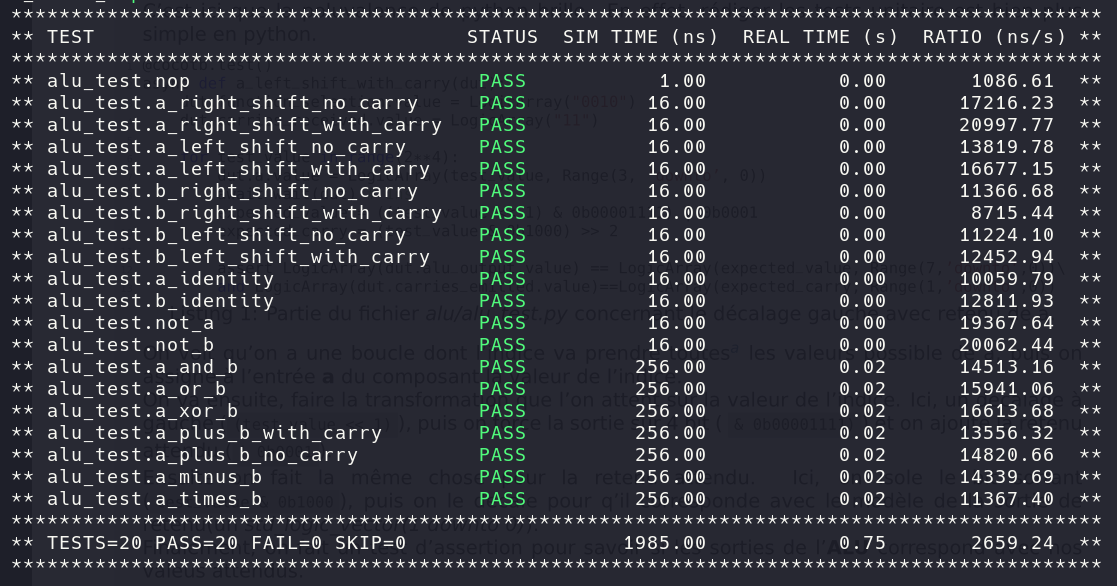
\includegraphics[width=0.7\textwidth]{alu/test_passed.png}
        \captionof{figure}{Confirmation du logiciel que tous les tests sont passés.}
      \end{center}
    }

    \question{dbus}{
      \begin{center}
        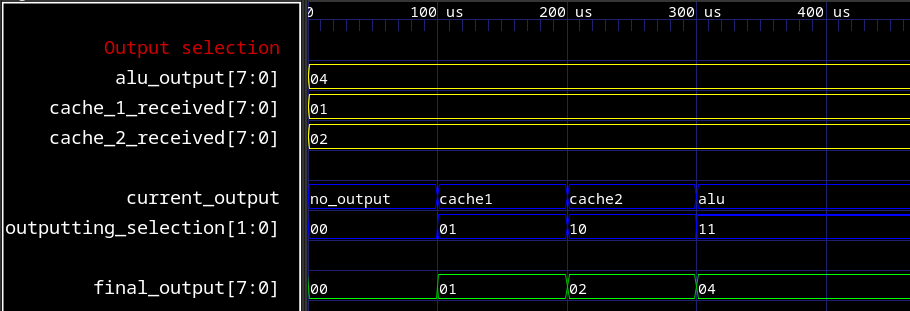
\includegraphics[width=0.75\textwidth]{dbus/out_sel.png}
        \captionof{figure}{Résultats visuels du dbus pour la partie de sélection de sortie.}
      \end{center}

      On a défini un signal auxiliaire pour une meilleure lisibilité. Il indique de quel composant la sortie va hériter.
      On voit que la sortie de l'interconnexion est bien contrôlée asynchroniquement par le signal \textbf{outputting\_selection}.

      \begin{center}
        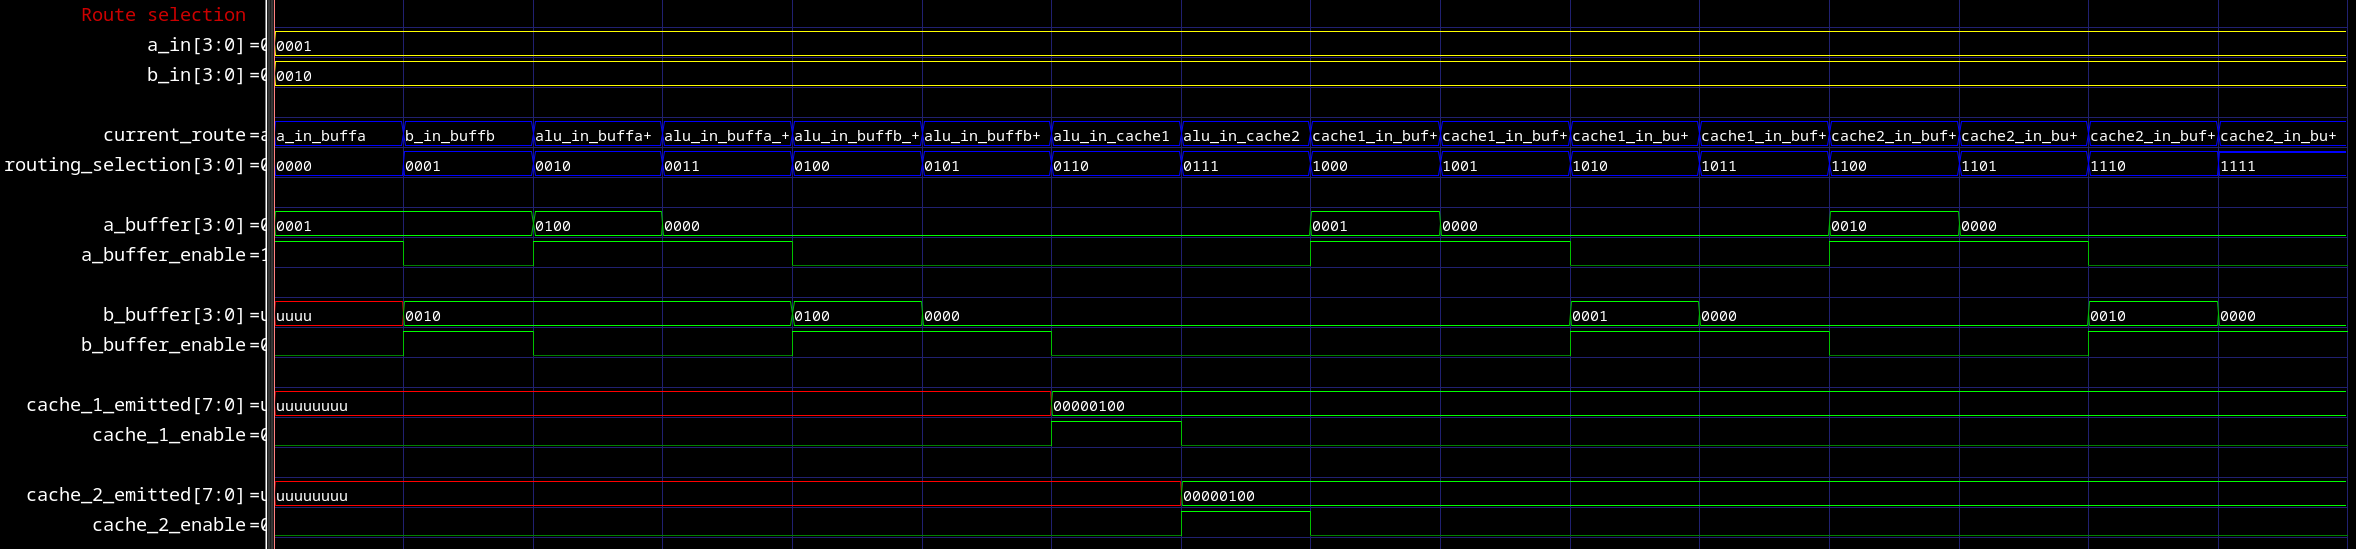
\includegraphics[width=\textwidth]{dbus/route_sel.png}
        \captionof{figure}{Résultats visuels du dbus pour la partie de sélection de route des données.}
      \end{center}

      On voit (assez peu précisément) que l'interconnexion contrôle bien la route des données.
      Par exemple les enable sont bien mise à un quand on a envie de modifier le buffer en question.

      Pour être plus exhaustif, je me remets aux tests unitaires.
      Ceux-ci sont rédigés comme suit.

      On a fixé les valeurs des entrées (\textbf{a\_in}, \textbf{b\_in}, \textbf{cache\_1\_received}, \textbf{cache\_2\_received}, \textbf{alu\_output}).

      \smallskip

      Puis on observe les sorties (\textbf{b\_buffer}, \textbf{a\_buffer\_enable}, \textbf{b\_buffer\_enable}, \textbf{cache\_1\_enable}, \textbf{cache\_2\_enable})
      pour détecter si le comportement est celui que l'on attend.

      \begin{center}
        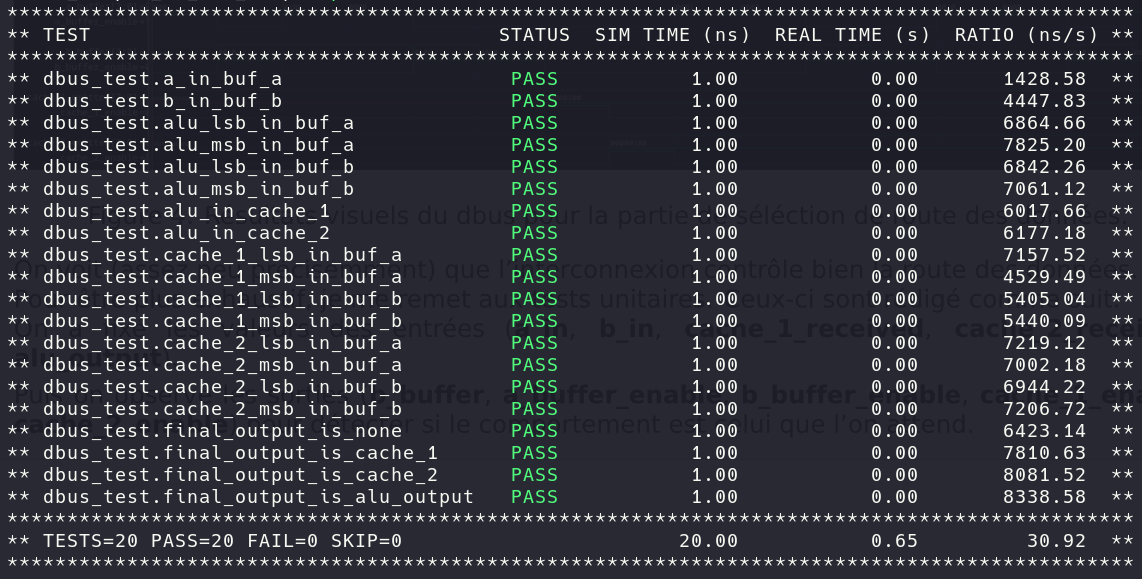
\includegraphics[width=0.7\textwidth]{dbus/test_passed.png}
        \captionof{figure}{Confirmation du logiciel que tous les tests sont passés.}
      \end{center}
    }

    \vfill

    \question{instructions}{
      \begin{center}
        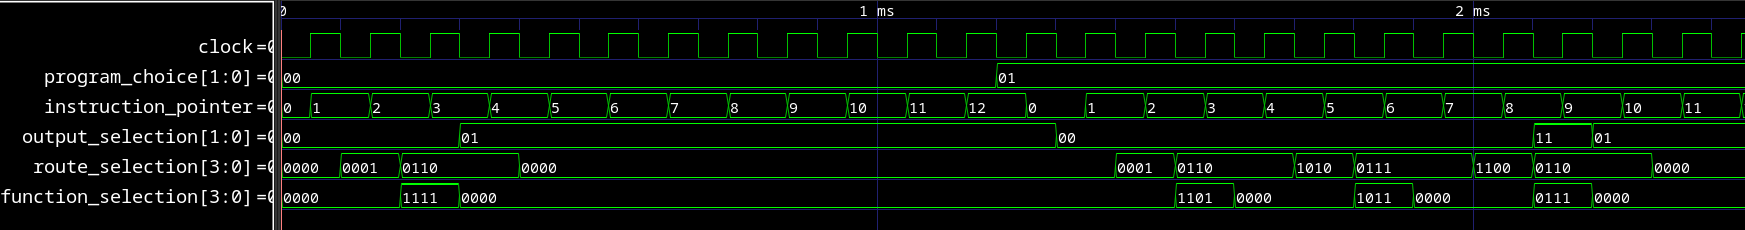
\includegraphics[width=\textwidth]{instructions/wave.png}
        \captionof{figure}{Sortie visuelle du bloc d'instruction des programmes res\_out\_1 et res\_out\_1 à 1200$\mu$s.}
      \end{center}

      \lstinputlisting[language=vhdl, caption={Instructions pour res\_out\_1, pour comparer.}]{images/instructions/res_out_1.sample}

      On voit bien que le bloc d'instruction envoie bien les commandes sur front descendant d'horloge.

      De plus, le pointeur d'instruction est bien remise à zéro quand on change de programme.
    }

    \question{nbuffer}{
      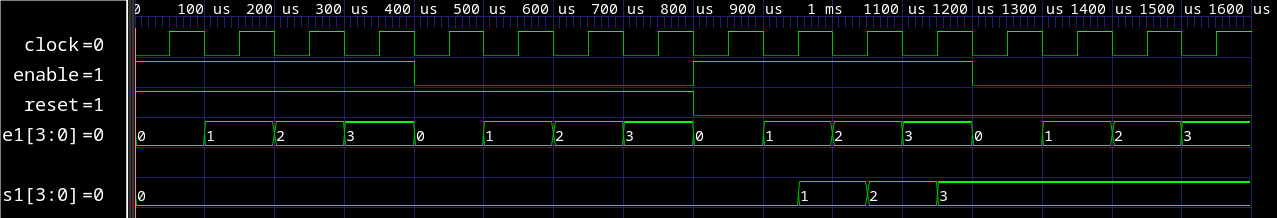
\includegraphics[width=\textwidth]{nbuffer.png}
      \captionof{figure}{Résultats visuels du buffer sur 2bit.}

      On voit que tout fonctionne comme entendu.
      
      Le signal \textbf{reset} force l'entrée à zéro.
      
      La sortie est bien sur front montant.

      Le signal \textbf{enable} permet la garde en mémoire, l'entrée précédente.
    }

    \vfill


    \pagebreak

    \question{LE RÉSULTAT FINAL}{
      On arrive enfin à la pièce maitresse du projet, le microcontrôleur.

      Dans le sujet, il nous est demandé de réaliser trois programmes pour le microcontrôleur.
      Comme indiqué précédemment, ils sont stockés dans le bloc d'instructions.

      J'ai suivi le même processus que pour l'ALU, et j'ai rédigé trois tests\footnote{Les plus durs à mettre en place.} exhaustifs avec un couvrage maximal.

      \lstinputlisting[language=python, caption={Test pour le programme res\_out\_1.}]{images/microcontroler/1.sample}

      Les trois ont la même forme.

      On va d'abord choisir le programme.

      Puis, on définit deux boucles qui vont être les valeurs des entrées du microcontrôleur.

      Ensuite, on les assigne et on attend le temps de calcul du résultat.

      Par la suite, nous appliquons le test d'assertion avec la valeur attendue calculée avec python.

      Enfin, on change de programme pour remettre à zéro le pointeur d'instruction.

      On remarque que les bornes sont signées, car le programme res\_out\_1 consiste en la multiplication, une instruction arithmétique.

      \medskip

      Pour le test du deuxième programme, on remarque que les bornes sont maintenant non signées, car le programme res\_out\_2 consiste en des transformations logiques.

      \medskip

      Nous avons la même chose pour le troisième programme, à l'exception que celui si à des bornes allant de 0 à 3 inclus pour les entrées.
      En effet, le programme ne concerne que les 2 premiers bit de chaque entrée.

      \begin{center}
        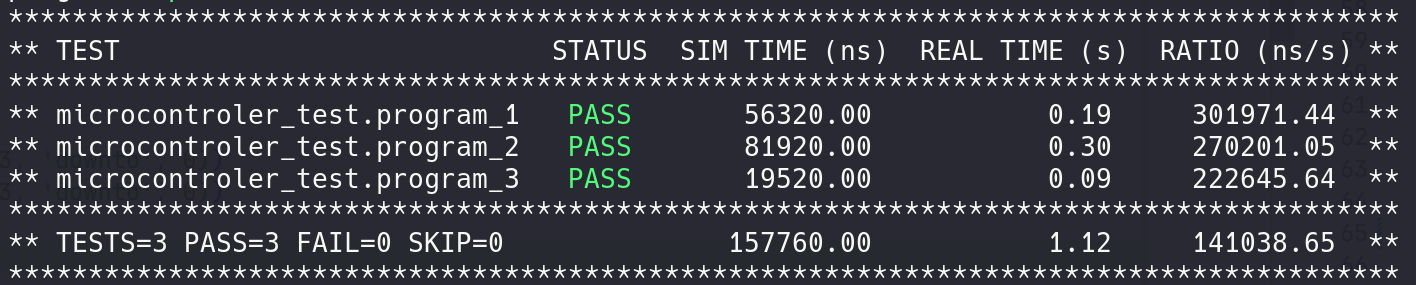
\includegraphics[width=0.7\textwidth]{microcontroler/tests_passed.png}
        \captionof{figure}{Confirmation du logiciel que tous les tests du microcontrôleur sont passés.}
      \end{center}\medskip

      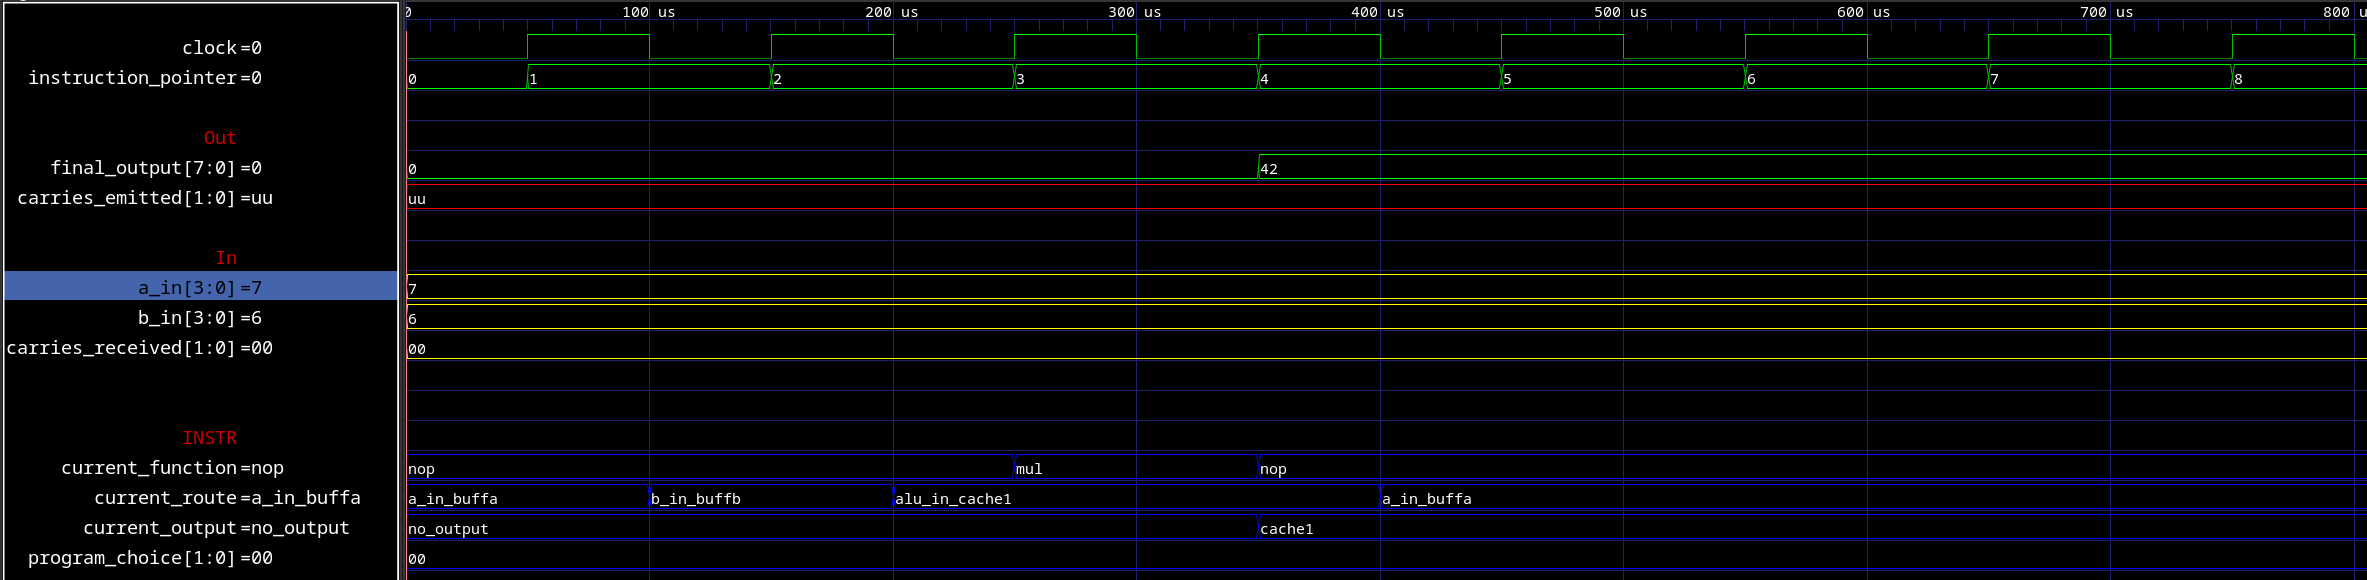
\includegraphics[width=\textwidth]{microcontroler/wave.png}
      \captionof{figure}{Rendu visuel montrant le programme 1 avec 6 et 7 en entrées.}\smallskip

      On peut voir que le résultat reste sur la sortie jusqu'au bout.
    }
  }

  \exercise{Conclusion}{
    \question[]{}{
      Je peux avec confiance, affirmé que le projet fonctionne. 
      
      De plus, nous avons eu l'opportunité d'expérimenter avec une carte FPGA\footnote{Xilinx Arty 35T}.
      J'y ai testé l'ALU du projet, qui fonctionnait.

      \medskip

      Tous les tests sont reproduisibles.
      Il suffit, comme indiqué en introduction, d'utiliser \textit{make}.
      
      Je conseillerais d'utiliser les tests pythons qui sont beaucoup plus exhaustifs et ayant un couvrage de toutes les possibilités.

      Vous trouverez tous les résultats de rendu et des tests dans les dossiers respectif de tous les composants.
      Les fichiers d'extension \inlinecode{.gtkw} sont déjà formatés par simplicité, il suffit de les ouvrir pour voir les signaux déjà organisés pour la visualisation.

      \medskip

      J'ai pu explorer en approfondissant mes nouvelles connaissances en VHDL et en programmation de FPGA.
    }
  }
\end{document}